In this Section, the results of the implementation of the machine learning algorithms on the binary classification dataset are presented. For each machine learning algorithm, the first step is to find the most suitable size of the moving window $m$ between $2$ (features only for the current day) and $100$ (size of the developed binary classification dataset). Note that $m$ can be regarded as a hyperparameter. If applicable, for each value of $m$ the intrinsic hyperparameters (such as K in the K-nearest neighbors algorithm) are optimized. The results are reported with suitable graphs and similar representations. Finally, for each machine learning algorithm, the performance in terms of prediction accuracy, sensitivity, and specificity on the test set is evaluated. \\

Besides the three machine learning algorithms described in the theory Section, also the performance of a simple majority predictor is evaluated. The majority predictor - that is a naive approach to solve the classification problem - is used as a reference for the performance of the other machine learning algorithms.

\subsection{Majority Predictor}
The majority predictor is a naive approach for solving the binary classfication problem. It constantly predicts the label that occurs most often in the training set, which in the present work is an increasing Bitcoin market price. Fig.~\ref{fig:major_acc_vs_m} reports the training accuracy (on the whole training set) and the 10-fold CV accuracy for the majority predictor as a function of the moving window length $m$. As expected, both accuracies are the same and coincide with the \SI{53.95}{\percent} labels \enquote{1} in the training set, see Fig.~\ref{fig:test}. There is also no dependence of the accuracy on the length $m$ of the moving window because the majority predictor depends only on the labels but not on the features of the examples in the training set. From this point of view, the majority predictor is a random classifier that classifies everything with a probability of \SI{100}{\percent} as \enquote{up}. \\

Tab.~\ref{tab:major_conf_mat} reports the confusion matrix of the majority predictor on the test set. Clearly, the majority predictor predicts only the majority label \enquote{1}. This explains also the sensitivity and specificity of the majority predictor in Tab.~\ref{tab:major_results}. The Table additionally reports the test accuracy of the majority predictor which is given by \SI{55.54}{\percent}. Again, this is simply the frequency of the label \enquote{1} in the test set, see Fig.~\ref{fig:test}.

\begin{figure}[h!]
  \centering
  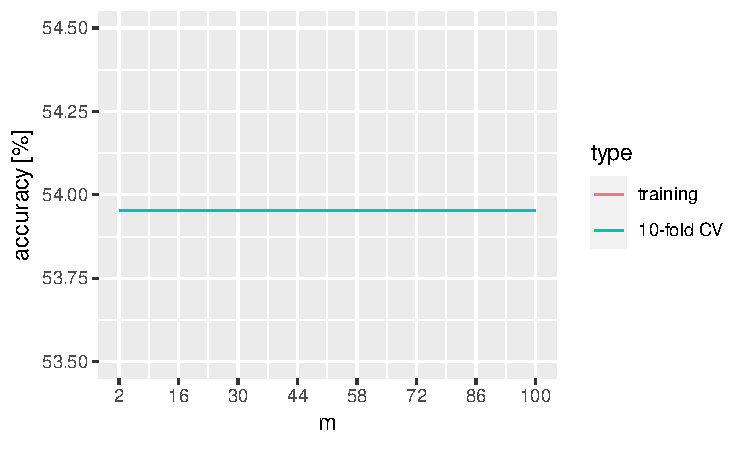
\includegraphics[width=0.8\textwidth]{major_acc_vs_m.pdf}
  \caption{Training and 10-fold CV accuracy of the majority predictor as a function of the moving window length $m$.}
  \label{fig:major_acc_vs_m}
\end{figure}

\begin{table}[h!]
\centering
\begin{tabular}{c|c|c|c|c}
  \backslashbox{predicted}{true} & $0$ & $1$ \\
 \hline
 $0$ & $0$ & $0$ \\  
 \hline
 $1$ & $309$ & $386$    
\end{tabular}
 \caption{Confusion matrix of the majority predictor on the test set.}
 \label{tab:major_conf_mat}
\end{table}

\begin{table}[h!]
\centering
\begin{tabular}{c|c|c}
accuracy [\%] & sensitivity [\%] & specificity [\%] \\
   \hline
$55.54$ & $100.00$ & $0.00$
\end{tabular}
 \caption{Accuracy, sensitivity, and specificity of the majority predictor on the test set.}
 \label{tab:major_results}
\end{table}

\subsection{Logistic Regression}
A more sophisticated algorithm compared to the majority predictor is the logistic regression. Fig.~\ref{fig:log_acc_vs_m} shows the training and 10-fold CV accuracy of the logistic regression fit as a function of the moving window length $m$. Besides $m$, there are no other hyperparameters to optimize. The 10-fold CV accuracy of the logistic regression fit is maximized for a moving window length of $m=4$. The training accuracy increases significantly with $m$. The main reason for this is that an increase of $m$ is equivalent to the inclusion of more features. The model uses these features to \enquote{store} the training examples, which leads to comparably high training accuracies. However, the general performance of the logistic regression does not improve with increasing $m$ as can be verified by the slightly decreasing 10-fold CV accuracy.\\

Fig.~\ref{fig:log_roc} shows the so-called receiver operating characteristic (ROC) curve of the logistic regression fit for $m=4$.

Recall that the logistic regression fit assigns a probability for the label \enquote{1} to all possible feature combinations. Predictions are made by applying a probability threshold. Typically, the threshold is set to \SI{50}{\percent}. 

The ROC curve displays the sensitivity and specificity for all possible values of the threshold from \SI{0}{\percent} in the upper righthand corner to \SI{100}{\percent} in the lower lefthand corner. E.g., for a threshold of $\SI{0}{\percent}$ everything is classified as \enquote{up}, and the majority predictor is obtained. As the majority predictor has a sensitivity of \SI{100}{\percent} and a specificity of \SI{0}{\percent}, it is located in the upper righthand corner of the ROC plot. The dashed diagonal line in the Figure is the ROC curve of a random classifier that does not make any use of information from the features. 

The ROC curve of the logistic regression fit lies above the random classifier which indicates a better sensitivitiy-specificity relation. This qualitative impression is quantified by the so-called area under the curve (AUC). For the random classifier the AUC is simply $0.5$, while the logistic regression fit obtains an AUC of $0.5486$.

\begin{figure}[h!]
  \centering
  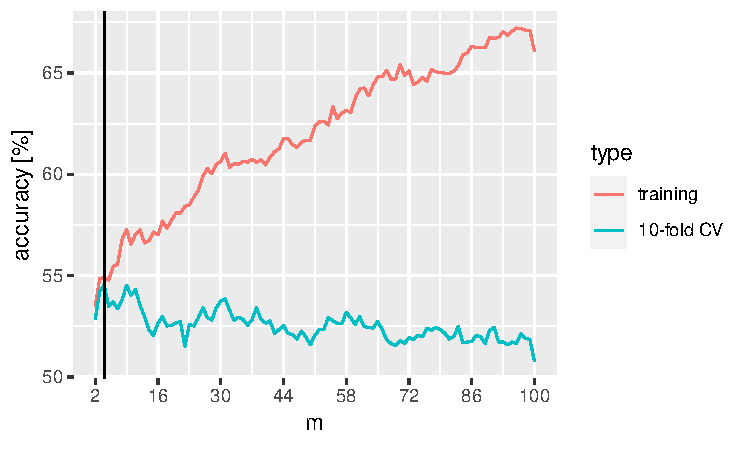
\includegraphics[width=0.8\textwidth]{log_acc_vs_m.pdf}
  \caption{Training and 10-fold CV accuracy of the logistic regression fit as a function of the moving window length $m$ for a prediction threshold of \SI{50}{\percent}. The vertical black line indicates the value of $m=4$ for which the 10-fold CV accuracy of the logistic regression fit is maximized.}
  \label{fig:log_acc_vs_m}
\end{figure}

\begin{figure}[h!]
  \centering
  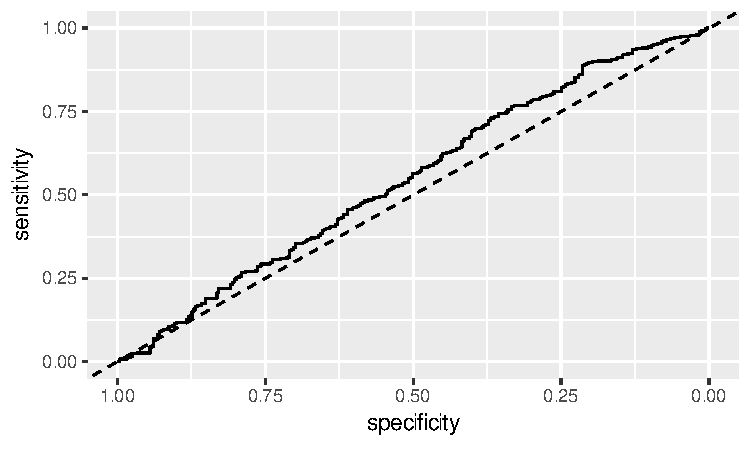
\includegraphics[width=0.8\textwidth]{log_roc.pdf}
  \caption{ROC curve of the logistic regression fit with a moving window length of $m=4$. The dashed diagonal line is the ROC curve of a random classifier that has an AUC of $0.5$. For the logistic regression fit, the AUC is $0.5486$.}
  \label{fig:log_roc}
\end{figure}

The confusion matrix of the logistic regression fit for $m=4$ with a threshold of \SI{50}{\percent} with respect to the test set, reported in Tab.~\ref{tab:log_conf_mat}, verifies the observation from the ROC plot and the AUC. Indeed, the logistic regression fit is able to classify both increasing and decreasing tomorrow's Bitcoin market prices correctly. In particular, the specificity is larger than \SI{0}{\percent}, as can been seen in Tab.~\ref{tab:log_results}. However, it is still significantly smaller than the sensitivity. So, the logistic regression fit predicts increasing Bitcoin market prices more often correctly than decreasing market prices.

\begin{table}[h!]
\centering
\begin{tabular}{c|c|c}
  \backslashbox{predicted}{true} & $0$ & $1$ \\
 \hline
 $0$ & $77$ & $73$ \\  
 \hline
 $1$ & $232$ & $313$    
\end{tabular}
 \caption{Confusion matrix of the logistic regression fit on the test set for a moving window length of $m=4$, and a prediction threshold of \SI{50}{\percent}.}
 \label{tab:log_conf_mat}
\end{table}

\begin{table}[h!]
\centering
\begin{tabular}{c|c|c}
accuracy [\%] & sensitivity [\%] & specificity [\%] \\
   \hline
$56.70$ & $81.09$ & $24.92$
\end{tabular}
 \caption{Accuracy, sensitivity, and specificity of the logistic regression fit on the test set for a moving window length of $m=4$, and a prediction threshold of \SI{50}{\percent}.}
 \label{tab:log_results}
\end{table}

Tab.~\ref{tab:log_coef} reports the coefficients of the logistic regression fit for a moving window length of $m=4$, and a prediction threshold of \SI{50}{\percent}. Almost all of the coefficients are not significant based on their relatively high standard deviation, and on the low $z$ scores close to zero. This has mainly two reasons. On the one hand, the actual relationship between the features and the label is not modeled correctly by the logistic regression. On the other hand, some of the features are correlated, as already observed in the development of the binary classification dataset. The influence of the correlation of the features on the standard deviatin of the estimated coefficients can be quantified by computing the so-called variance inflation coefficients (VIF). In Tab.~\ref{tab:log_vif}, the square-root of the VIF coefficients for all of the estimated logistic regression coefficients are reported. The square-root of the VIF indicates how much larger the standard deviation of each estimated coefficient is compared to the case where there were no correlation between the features. Typically, a value of about $2$ is taken as a threshold for a negligible influence of feature correlation. It is observed that especially the estimated coefficients related to the Bitcoin market price have a high VIF. This is caused by the high autocorrelation of the Bitcoin market price for lags smaller than $100$
days, and is actually desired for a prediction of tomorrow's Bitcoin market price. 

All in all, the fact that the binary classification is not modelled correctly by the logistic regression, and the poor statistics make a statistical inference from the coefficients difficult. It cannot be deduced which feature is responsible for an increasing Bitcoin market price, and which for a decreasing market price because the feature correlation makes the logistic regression fit results unstable. However, the logistic regression model can still be used to make predictions, and its performance can be evaluated on the independent test set.

\begin{table}[h!]
\centering
\begin{tabular}{c||c|c|c|c}
coefficient & estimate & std. & $z$ score & $P(>|z|)\,[\%]$ \\
 \hline
 \hline
(intercept) & $-0.15$ & $0.22$ & $-0.688$ & $49.13$ \\  
 \hline
 market price ($t_{-2}$) & $0.45$ & $-0.60$ & $0.764$ & $44.51$\\   
 \hline
market price ($t_{-1}$) & $0.71$ & $0.82$ & $0.874$ & $38.20$\\
\hline
market price ($t_{0}$) & $-0.65$ & $0.57$ & $-1.121$ & $26.22$\\
\hline
\# transactions ($t_{-2}$) & $-0.28$ & $0.27$ & $-1.040$ & $29.81$\\
\hline
\# transactions ($t_{-1}$) & $0.20$ & $0.32$ & $0.624$ & $53.28$\\
\hline
\# transactions ($t_{0}$) & $0.11$ & $0.27$ & $0.394$ & $69.32$\\
\hline
avg. block size ($t_{-2}$) & $-0.10$ & $0.28$ & $-0.252$ & $80.10$\\
\hline
avg. block size ($t_{-1}$) & $-0.54$ & $0.32$ & $-1.682$ & $9.25$\\
\hline
avg. block size ($t_{0}$) & $0.69$ & $0.28$ & $2.501$ & $1.24$\\
\hline
hash rate ($t_{-2}$) & $-0.10$ & $0.26$ & $-0.171$ & $86.44$\\
\hline
hash rate ($t_{-1}$) & $-0.10$ & $0.28$ & $-0.043$ & $96.56$\\
\hline
hash rate ($t_{0}$) & $-0.10$ & $0.26$ & $-0.029$ & $97.67$\\
\end{tabular}
 \caption{Estimated coefficients of the logistic regression fit for a moving window length of $m=4$, and a prediction threshold of \SI{50}{\percent}. For each coefficient, the standard deviation, the $z$ score, and the probability to obtain a $z$ score with an absolute value larger than the obtained one based on the $z$ statistic are given.}
 \label{tab:log_coef}
\end{table}

\begin{table}[h!]
\centering
\begin{tabular}{c|c}
coefficient & $\sqrt{VIF}$ \\
 \hline
 \hline
 market price ($t_{-2}$) & $4.69$ \\   
 \hline
market price ($t_{-1}$) & $6.64$ \\
\hline
market price ($t_{0}$) & $4.82$ \\
\hline
\# transactions ($t_{-2}$) & $1.68$ \\
\hline
\# transactions ($t_{-1}$) & $2.01$ \\
\hline
\# transactions ($t_{0}$) & $1.70$ \\
\hline
avg. block size ($t_{-2}$) & $1.78$ \\
\hline
avg. block size ($t_{-1}$) & $2.08$ \\
\hline
avg. block size ($t_{0}$) & $1.79$\\
\hline
hash rate ($t_{-2}$) & $1.45$ \\
\hline
hash rate ($t_{-1}$) & $1.55$ \\
\hline
hash rate ($t_{0}$) & $1.46$ \\
\end{tabular}
 \caption{Square-root of the VIF for all of the estimated coefficients in the logistic regression fit from Tab.~\ref{tab:log_coef}. Typically, a value of about $2$ is taken as a threshold for a negligible influence of the correlation between the features.}
 \label{tab:log_vif}
\end{table}

\clearpage
\subsection{K-Nearest Neighbors Algorithm}
The next algorithm that is trained on the binary classification dataset is the K-nearest neighbors algorithm. The K-nearest neighbors algorithm has the hyperparameter K - the number of nearest neighbors that is considered for each prediction. Thus, for each moving window length $m$, additionally the hyperparameter K is optimized via 10-fold CV. The optimal hyperparameter $K_{max}$ that maximizes the 10-fold CV for each moving window length $m$ is reported in Fig.~\ref{fig:knn_K_max}. Fig.~\ref{fig:knn_acc_vs_m} shows the accuracies of the best predictor using $K_{max}$ for each moving window length $m$. The highest 10-fold CV accuracy is obtained for $m=91$ using $K_{max}=29$. Whenever, the highest 10-fold CV accuracy is obtained with $K_{max}=1$, the training accuracy is \SI{100}{\percent}.\\

For $m=91$, Fig.~\ref{fig:knn_acc_vs_K} shows the search for the optimal hyperparameter explicitly. As expected, the training accuracy is always larger than the 10-fold CV accuracy, and drops significantly for an increasing number K of nearest neighbors. The 10-fold CV accuracy increases slightly with K which indicates a higher prediction performance. The optimal value of K is obtained when the 10-fold CV accuracy is maximized. Here, this is the case for $K_{max}=29$.

\begin{figure}[h!]
  \centering
  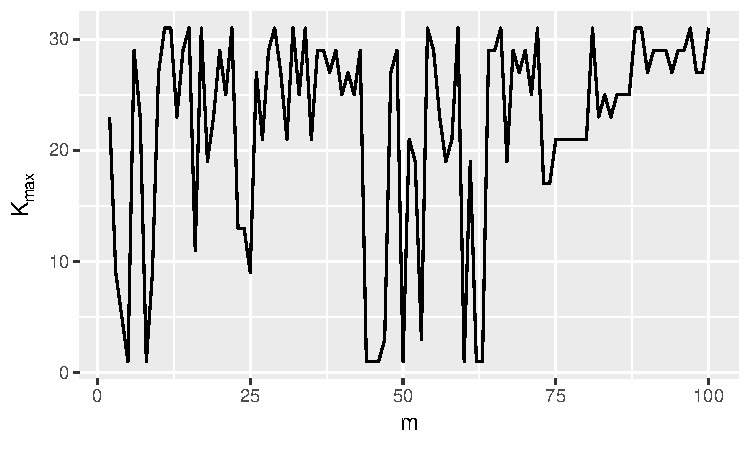
\includegraphics[width=0.8\textwidth]{knn_K_max.pdf}
  \caption{Number of nearest neighbors $K_{max}$ for which the 10-fold CV accuracy using a prediction threshold of \SI{50}{\percent} for each moving window length $m$ is maximized.}
  \label{fig:knn_K_max}
\end{figure}

\begin{figure}[h!]
  \centering
  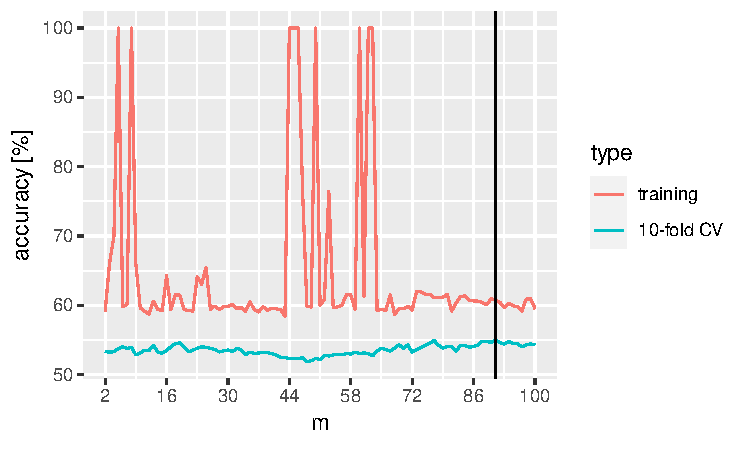
\includegraphics[width=0.8\textwidth]{knn_acc_vs_m.pdf}
  \caption{Training and 10-fold CV accuracy for the K-nearest neighbors algorithm as a function of the moving window length $m$ for a prediction threshold of \SI{50}{\percent}. For each $m$, the accuracies for the optimal number of nearest neighbors $K_{max}$ from Fig.~\ref{fig:knn_K_max} is reported. The vertical black line indicates the value of $m=91$ for which the 10-fold CV accuracy of the K-nearest neighbors regression using $K_{max}=29$ is maximized.}
  \label{fig:knn_acc_vs_m}
\end{figure}

\begin{figure}[h!]
  \centering
  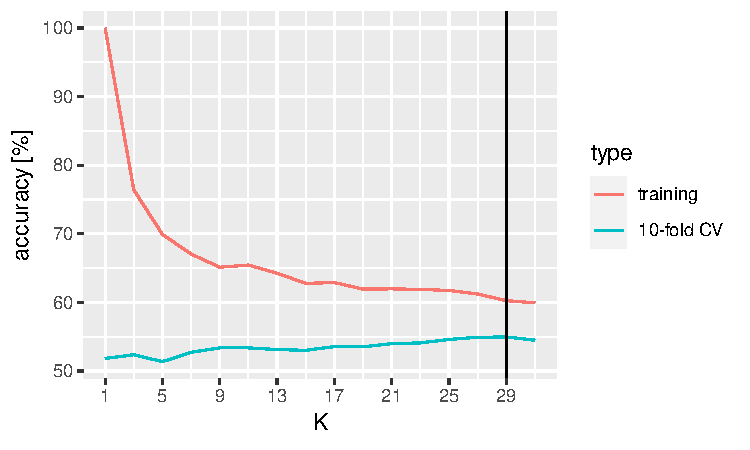
\includegraphics[width=0.8\textwidth]{knn_acc_vs_K.pdf}
  \caption{Training and 10-fold CV accuracy for the K-neareast neighbors algorithm as a function of $K$ for the optimal moving window size $m=91$ using a prediction threshold of \SI{50}{\percent}. The vertical black line indicates the value of $K_{max} = 29$ for which the 10-fold CV accuracy of the K-nearest neighbors algorithm is maximized.}
  \label{fig:knn_acc_vs_K}
\end{figure}

Similar to the analysis of the logistic regression fit in the last Subsection, Fig.~\ref{fig:knn_roc} shows the ROC curve of the K-nearest neighbors algorithm for $m=91$ and $K_{max}=29$ for different prediction thresholds in comparison to a random classifier. The ROC curve of the K-nearest neighbors algorithm lies only slightly above the ROC curve of a random classifier. In addition, the K-nearest neighbor algorithms leads to an AUC of only $0.5038$. Thus, the K-nearest neigbor algorithm performs only slightly better than a random classifier. 

The confusion matrix of the K-nearest neighbors algorithm is reported in Tab.~\ref{tab:knn_conf_mat}. The prediction accuracy, sensitivity, and specficitiy of the K-nearest neighbors algorithm is summarized in Tab.~\ref{tab:knn_results}. Also the test accuracy of \SI{51.80}{\percent} is only slightly higher than \SI{50}{\percent}.

\begin{figure}[h!]
  \centering
  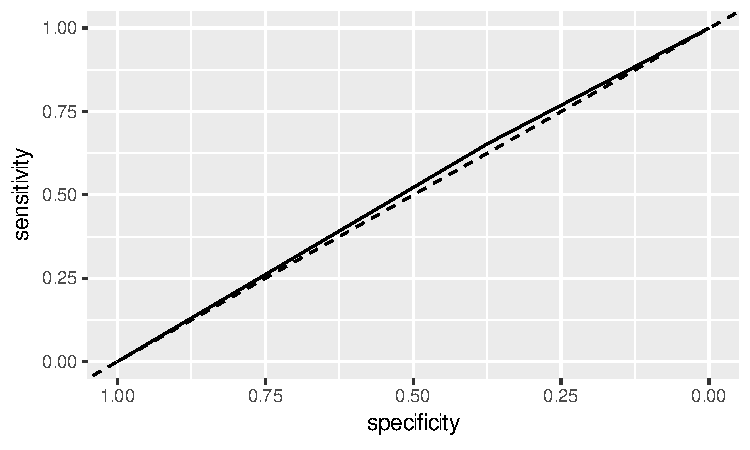
\includegraphics[width=0.8\textwidth]{knn_roc.pdf}
  \caption{
ROC curve of the K-nearest neighbors algorithm with a moving window length of $m=91$, and $K_{max} = 29$. The dashed diagonal line is the ROC curve of a random classifier that has an AUC of $0.5$. For the K-nearest neighbors algorithm, the AUC is $0.5038$.}
  \label{fig:knn_roc}
\end{figure}

\begin{table}[h!]
\centering
\begin{tabular}{c|c|c}
  \backslashbox{predicted}{true} & $0$ & $1$ \\
 \hline
 $0$ & $115$ & $133$ \\  
 \hline
 $1$ & $194$ & $253$    
\end{tabular}
 \caption{Confusion matrix of the K-nearest neighbors algorithm on the test set for a moving window length of $m=91$, $K_{max}=29$, and a prediction threshold of \SI{50}{\percent}.}
 \label{tab:knn_conf_mat}
\end{table}

\begin{table}[h!]
\centering
\begin{tabular}{c|c|c}
accuracy [\%] & sensitivity [\%] & specificity [\%] \\
   \hline
$51.80$ & $65.54$ & $37.21$
\end{tabular}
 \caption{Accuracy, sensitivity, and specificity of the K-nearest neighbors algorithm on the test set for a moving window length of $m=4$, $K_{max}=29$, and a prediction threshold of \SI{50}{\percent}.}
 \label{tab:knn_results}
\end{table}

\subsection{Deep Neural Network}

The last machine learning algorithm applied on the binary classification dataset is a deep neural network. The results in this Subsection refer to a deep neural network with four hidden layers with the following number of neurons: $20$-$30$-$20$-$10$. This amounts to a total of $ 5962$ trainable parameters. However, several other architectures - varying in the number of hidden layers and the number of neurons - lead to the same results.\\

The training of the deep neural network depends on the number of epochs $N_{epoch}$ over the whole training set. Fig.~\ref{fig:dnn_N_max} reports the optimal number of epochs $N_{epoch,max}$ for each moving window length $m$. For the evaluation of the deep neural network, the simple \textit{training-, validation-, and test-set} approach is used for computational reasons. Almost for all values of $m$ the maximum validation accuracy is reached for a small number of epochs $N_{epoch,max}$ of the order of $1$ and $2$. This indicates that the training of the deep neural network does not improve its performance.\\

This impression is verified when looking examplarily at the training and validation accuracies of the deep neural network for a moving window length of $m=57$ as a function of the number of epochs $N_{epoch}$, see Fig.~\ref{fig:dnn_acc_vs_N}. It is observed that both the training and validation accuracies saturate after $N_{epoch} = 3$ epochs. The validation accuracy is actually the fraction of the examples in the validation set that are labeled with \enquote{1}. The training accuracy is smaller than the validation accuracy because dropout with a rate of $0.5$ between all layers of the deep neural network is applied. \\

Fig.~\ref{fig:dnn_acc_vs_m} reports the training and validation accuracy for the deep neural network as a function of the moving window length $m$ for the optimal epoch numbers in Fig.~\ref{fig:dnn_N_max}. The Figure shows that the observed phenomenon takes place for all values of $m$. \\

Tab.~\ref{tab:dnn_conf_mat} and Tab.~\ref{tab:dnn_results} report the confusion matrix as well as the prediction accuracy, the sensitivity, and the specificity of the deep neural network on the test set. The obtained results show that the deep neural network reproduces the majority predictor, and does not lead to an improvement over the logistic regression fit, and the K-nearest neighbors algorithm.

\begin{figure}[h!]
  \centering
  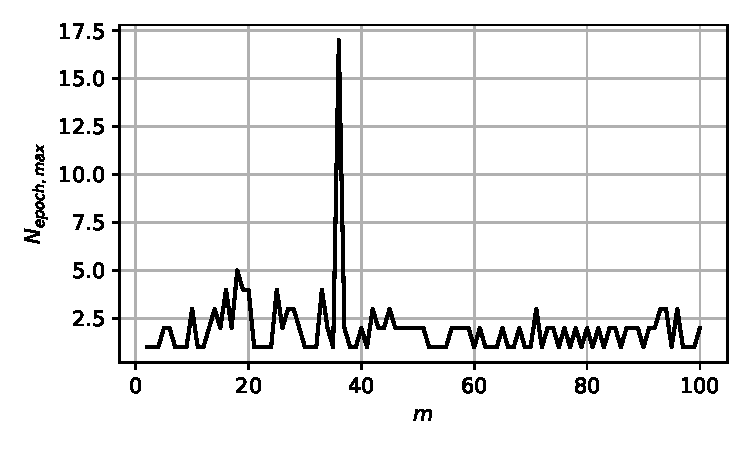
\includegraphics[width=0.8\textwidth]{dnn_N_max.pdf}
  \caption{Number of epochs $N_{epoch,max}$ for which the validation accuracy using a prediction threshold of \SI{50}{\percent} for each moving window length $m$ is maximized.}
  \label{fig:dnn_N_max}
\end{figure}

\begin{figure}[h!]
  \centering
  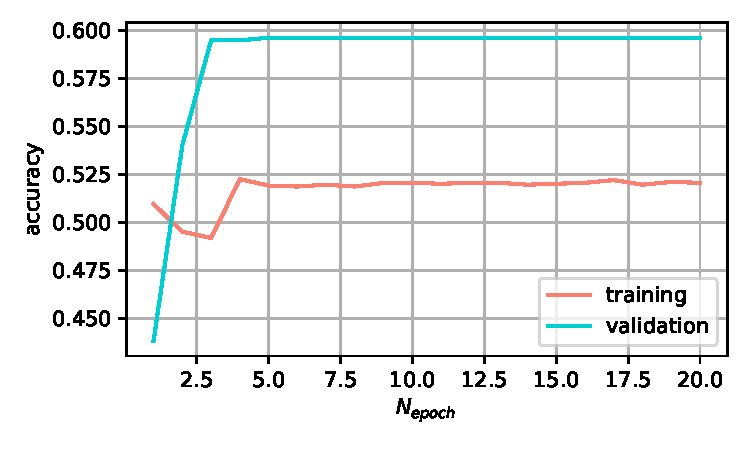
\includegraphics[width=0.8\textwidth]{dnn_acc_vs_N.pdf}
  \caption{Training and validation accuracy of the deep neural network as a function of $N_{epoch}$ for a moving window length of $m=57$ using a prediction threshold of \SI{50}{\percent}.}
  \label{fig:dnn_acc_vs_N}
\end{figure}

\clearpage

\begin{figure}[h!]
  \centering
  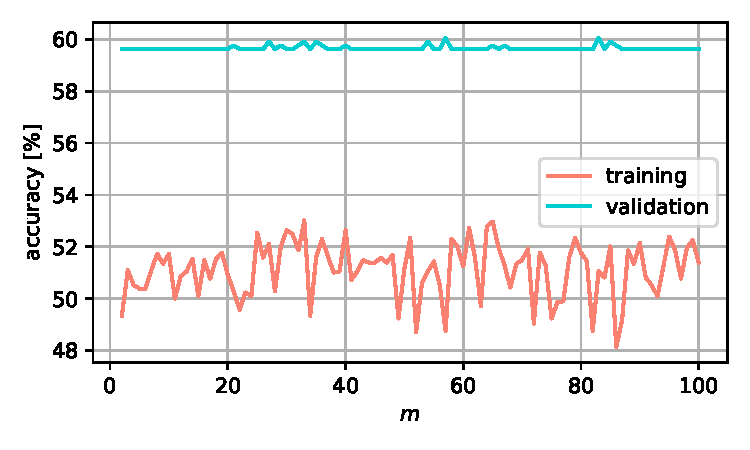
\includegraphics[width=0.8\textwidth]{dnn_acc_vs_m.pdf}
  \caption{Training and validation accuracy of the deep neural network as a function of the moving window length $m$ for a prediction threshold of \SI{50}{\percent}. The accuracies for the optimal epoch numbers in Fig.~\ref{fig:dnn_N_max} are reported.}
  \label{fig:dnn_acc_vs_m}
\end{figure}

\begin{table}[h!]
\centering
\begin{tabular}{c|c|c}
  \backslashbox{predicted}{true} & $0$ & $1$ \\
 \hline
 $0$ & $0$ & $0$ \\  
 \hline
 $1$ & $309$ & $386$    
\end{tabular}
 \caption{Confusion matrix of the deep neural network on the test set for a moving window length of $m=57$, $N_{epoch, max}=3$, and a prediction threshold of \SI{50}{\percent}. The deep neural network reproduces the confusion matrix of the majority predictor.}
 \label{tab:dnn_conf_mat}
\end{table}

\begin{table}[h!]
\centering
\begin{tabular}{c|c|c}
accuracy [\%] & sensitivity [\%] & specificity [\%] \\
   \hline
$55.54$ & $100.00$ & $0.00$
\end{tabular}
 \caption{Accuracy, sensitivity, and specificity of the deep neural network on the test set for a moving window length of $m=53$, $N_{epoch, max}=3$, and a prediction threshold of \SI{50}{\percent}. The deep neural network reproduces the values of the majority predictor.} 
 \label{tab:dnn_results}
\end{table}